\def\r{3em}
\def\angle{10}
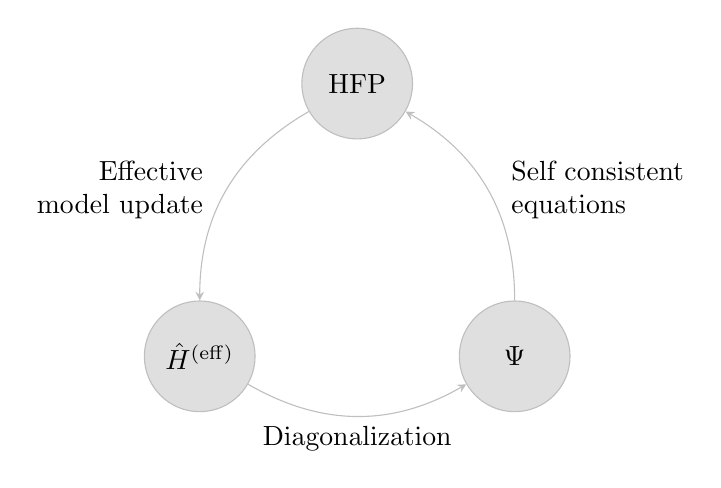
\begin{tikzpicture} 
	
    \node[
        name=he,
        circle,
        draw=lightgray,
        text=black,
        fill=lightgray!50,
        minimum size=4em
    ] 
        (He) at (0,0)
            {$\hat H^{(\mathrm{eff})}$};
            
    \node[
        name=psi,
        circle,
        draw=lightgray,
        text=black,
        fill=lightgray!50,
        minimum size=4em
    ] 
        (PSI) at (4,0)
            {$\ket{\Psi}$};
            
    \node[
        name=hfp,
        circle,
        draw=lightgray,
        text=black,
        fill=lightgray!50,
        align=center,
        minimum size=4em
    ] 
        (HFP) at (2,3.464)
            {HFP};
            
    \draw[color=lightgray, -stealth]
        (He) to[bend right]node[below,color=black]{Diagonalization} (PSI);
    \draw[color=lightgray, -stealth]
        (PSI) to[bend right]node[right,color=black,align=left,xshift=0.5em]{Self consistent\\equations} (HFP);
    \draw[color=lightgray, -stealth]
        (HFP) to[bend right]node[left,color=black,align=right,xshift=-0.5em]{Effective\\model update} (He);

\end{tikzpicture}
